% !TeX spellcheck = de_DE
\documentclass{alex_gp}

\name{Alexander Helbok}
\course{Grundpraktikum}
\hwnumber{4}
\spacing{2.5}

\begin{document}


\begin{mybox}{Laufzeitmessung}
	Ziel dieses Versuches ist es, die Schallgeschwindigkeit in der Luft mittels einer Laufzeitmessung zu bestimmen. Dazu wurde eine Lichtquelle (Taschenlampe) und das Messgerät auf einem Tisch positioniert und in einem Abstand von \( d = 3 \unit{m} \) vom IOLab wurde eine Markierung am Tisch vorgenommen. An dieser Markierung wurde mit einem Brett der Lichtstrahl unterbrochen und gleichzeitig am Tisch ein lautes Geräusch erzeugt. Beide Signale kommen am IOLab an, wobei der Schlag vom Brett zeitlich leicht verzögert ankommt, da die Geschwindigkeit des Schalls wesentlich kleiner als die des Lichts ist. Aus dieser Zeitdifferenz lässt sich die Schallgeschwindigkeit berechnen. 
	
	Für die Distanz wurde ein Fehler von \( 1 \unit{cm} \) angenommen, um für den Ablesefehler, die Genauigkeit beim Herunterschlagen der Brettes und die Positionierung des Sensors im IOLab zu kompensieren. Die Daten wurden bei einer Abfragerate von \( 2400 \unit{Hz} \) aufgezeichnet, weshalb die Unsicherheit in der Zeit auf \( 1/(2\cdot2400) \unit{1/Hz} = 0.21 \unit{µs} \) geschätzt wurde.
	
	\begin{figure}[H]	
		\centering
		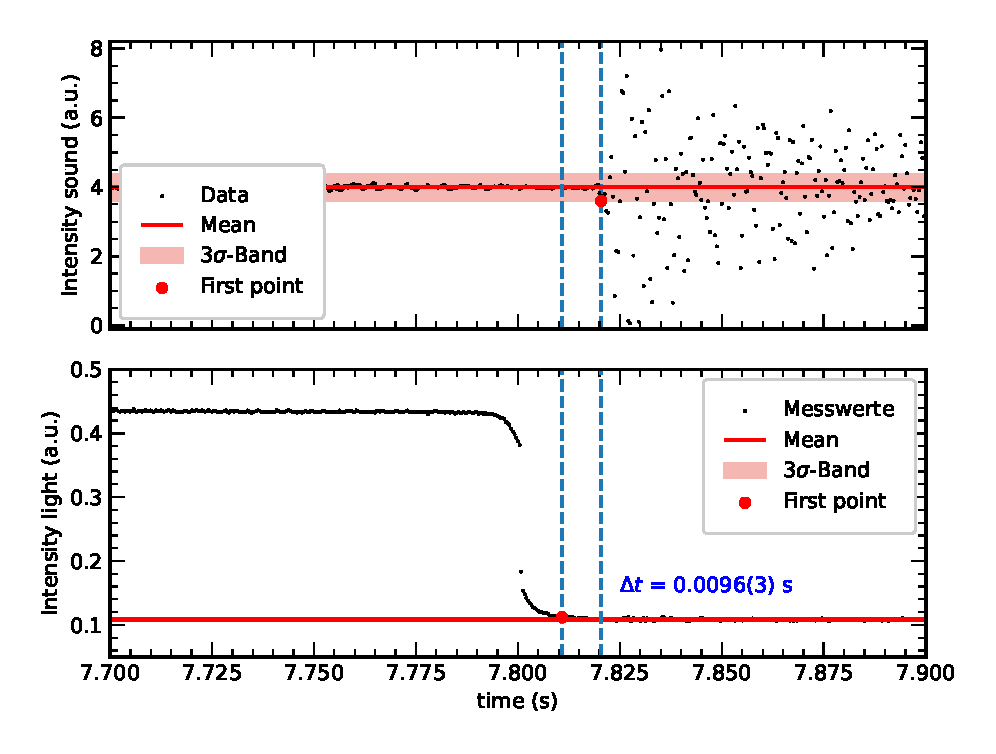
\includegraphics[width=\textwidth]{Versuch4_1.eps}
		\caption{Von oben nach unten sind Intensität des Schalls und des Lichts auf die Zeit aufgetragen. Die Daten werden ohne Fehlerbalken dargestellt, da diese zu klein wären. In Rot wurde der Mittelwert mit \( 3\sigma \)-Band aufgetragen und in blau ist die Zeitdifferenz zwischen den ersten beiden roten Punkten zu sehen.}
		\label{fig:laufzeit}
	\end{figure}

	Die Analyse der Daten ging wie folgt: es wurde zuerst der Mittelwert des Audiosignals vor dem Schlagereignis und der Mittelwert der Lichtintensität nach dem Schlagereignis berechnet. Das Audiosignal wird als registriert angenommen, wenn der erste Wert mehr als \( 3\sigma \) vom Mittelwert abweicht, da die Wahrscheinlichkeit, dass dies durch Zufall eintrifft klein genug ist (\( 0.3 \% \)). Analog gilt das Lichtsignal als Unterbrochen sobald der erste Datenpunkt der Lichtmessung mehr also \( 3\sigma \) vom Mittelwert abweicht. 
	
	Dieser Prozess ist in \autoref{fig:laufzeit} dargestellt, wo die Mittelwerte „in Ruhe“ als horizontale Linien aufgetragen sind. Der erste Datenpunkt, der mehr als \( 3\sigma \) abweicht, und somit außerhalb der roten Konfidenzbandes liegt, wurde rot markiert. Durch die beiden roten Punkte gehen vertikale blaue Linien, aus welchen sich \( \Delta t \) durch Subtraktion berechnet.

	Die Zeitdifferenz \( \Delta t \) zwischen dem unterbrechen des Lichtstrahls und dem Ankommen der Schallwelle beim Messgerät kann nun herangezogen werden, um die Schallgeschwindigkeit wie folgt zu berechnen
	\begin{equation}\label{eqn:v1}
		v = \frac{d}{\Delta t}
	\end{equation}

	Die Messung wurde Fünf man wiederholt und in \autoref{fig:vmean} wurden die berechneten Geschwindigkeiten als normalisierte Gaußkurven auf die Geschwindigkeit aufgetragen. Es sind nur 3 Gaußkurven zu sehen, da aus drei Messungen die gleiche Geschwindigkeit berechnet wurde und diese daher als kombinierte (und höhere) Normalverteilungskurve dargestellt werden. In Rot ist die Überlagerung der Messungen als bester Schätzwert der Schallgeschwindigkeit dargestellt, wobei dessen Fehler gerade dem 1$\sigma$ Konfidenzintervall der Gaußkurve ist und farblich hervorgehoben wurde,
	\begin{figure}[H]	
		\centering
		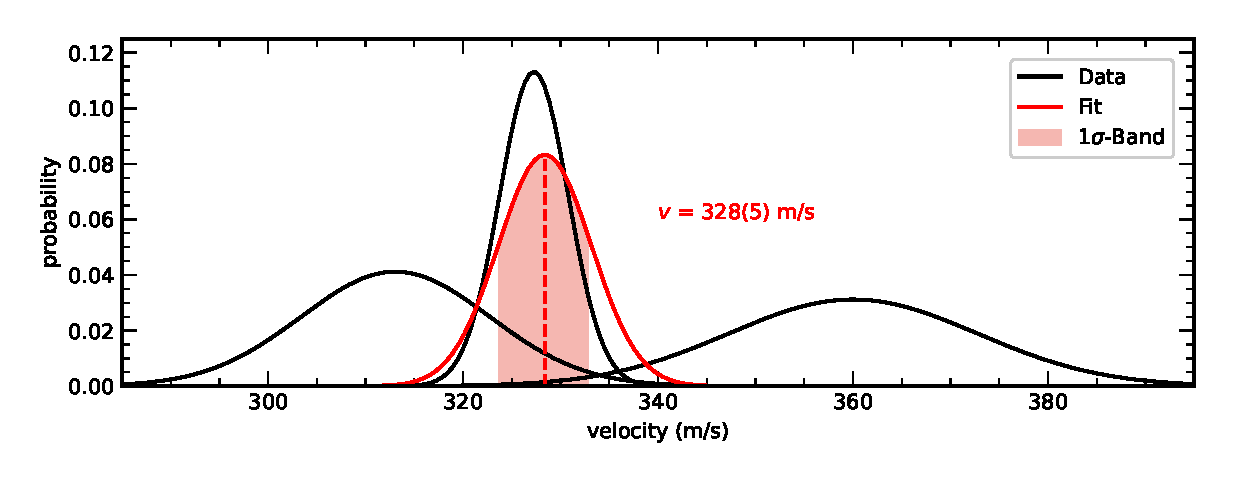
\includegraphics[width=\textwidth]{Versuch4_2.eps}
		\caption{Die gemessenen Geschwindigkeiten wurden als normalisierte Gaußkurven in schwarz auf die Geschwindigkeiten aufgetragen. In Rot der gewichtete Mittelwert, der sich als Überlagerung (und anschließende Normalisierung) der schwarzen Kurven ergibt. Das \( 1\sigma \) Intervall des Mittelwerts wurde farblich hinterlegt.}
		\label{fig:vmean}
	\end{figure}

	Die Laufzeitmessung liefert für die Schallgeschwindigkeit in Luft einen Wert von \( v = 328(5) \unit{\v} \). Dieser Wert liegt etwas unter dem vorhergesagten Wert (Siehe Seite \pageref{eqn:cad}), weicht aber nicht signifikant davon. 
	
	Um den statistischen Fehler der Messung zu reduzieren müsste man mit mehr Auflösung messen, also mehr Datenpunkte pro Zeitintervall aufnehmen, da der statistische Fehler in \( v \) zu über \( 99 \% \) daher stammt. Der Versuchsaufbau war nicht optimal, wodurch sich systematische Fehler eingeschlichen haben. Es entsteht eine zeitliche Verzögerung dadurch, dass das Audiosignal erst erzeugt wird, nachdem das Lichtsignal unterbrochen ist
\end{mybox}

\begin{mybox}{Resonanzmessung}
	Dieser Versuch macht sich das Resonanzverhalten von Schallwellen zunutze, um einen Wert für dessen Geschwindigkeit zu erhalten.
	Dafür wurde ein Kartonrohr der Länge \newline\( L = 81.60(10) \unit{cm} \) und einem Durchmessen \( d = 0.40(10) \unit{cm} \) hergenommen. Ein Ende wurde mit dem IOLab abgedichtet und das Andere wurde offen gelassen und über Kopfhörer Töne reingespielt. Da das Rohr an einem Ende offen, muss man Korrekturen an der Länge vornehmen, sodass für die effektive Länge gilt \( L_{\text{eff}} = L + 0.6d = 81.84(12) \unit{cm} \).
	
	Die von den Lautsprechern erzeugten Schallwellen werden am geschlossenen Ende des Rohres reflektiert und interferieren mit den gegenläufigen Schwingungen. Bei bestimmten Frequenzen interferieren die Wellen maximal konstruktiv und es kommt zu stehenden Wellen. Aus der Schwingungsgleichung für Druckwellen kann man sich die Frequenzen ausrechnen, bei welchen stehende Wellen entstehen und man erhält \( f_n = (2n+1)v/4L_{\text{eff}} \) beziehungsweise für aufeinanderfolgende Frequenzen \( f_{\text{n+1}} - f_{\text{n}} = v/2L_{\text{eff}} \)
%    \begin{equation}\label{eqn:fn}
%    	f_{\text{n+1}} - f_{\text{n}} = \frac{v}{2L_{\text{eff}}}
%    \end{equation}
	Hier haben wir eine Beziehung zwischen den Resonanzfrequenzen, der Länge des Rohren und der Schallgeschwindigkeit. Formen wir das nun auf \( v \) um, erhält man
	\begin{equation}\label{eqn:cfn}
		v = \left(f_{\text{n+1}} - f_{\text{n}}\right) 2L_{\text{eff}}
	\end{equation}

	Die Resonanzmaxima und die dazugehörigen Frequenzen wurden wie folgt aus den Daten extrahiert: um das oszillierende Audiosignal wurde eine einhüllende Funktion gelegt, aus welcher die lokalen Maxima bestimmt wurden. An den Extremstellen wurden Fouriertransformationen durchgeführt. Die Fehler der Maxima wurden über die Breite der Resonanzmaxima abgeschätzt, werden aber nach der Transformation so gering (im Vergleich zum Fehler der Rohrlänge), dass sie vernachlässigbar sind. 
	
	\begin{figure}[H]	
		\centering
		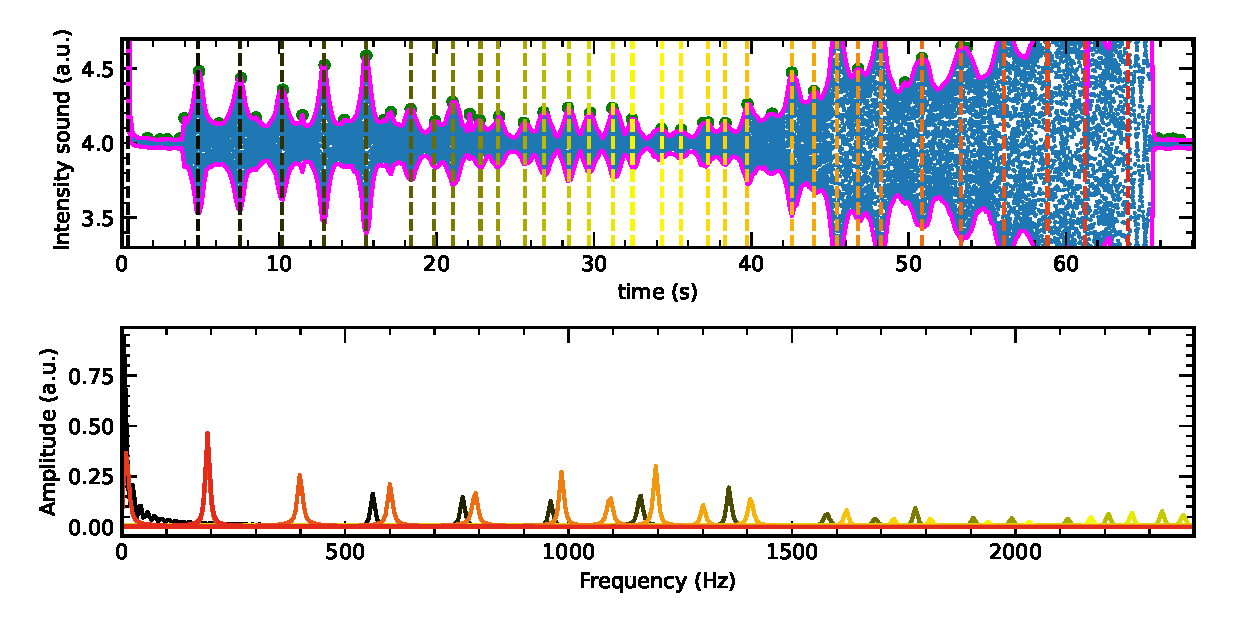
\includegraphics[width=\textwidth]{Versuch4_3.eps}
		\caption{Links oben ist das Audiosignal auf die Zeit von \( t = 4 \unit{s} \) bis \( t = 16.4 \unit{s} \) aufgetragen; rechts oben von \( t = 44.5 \unit{s} \) bis \( t = 60.2 \unit{s} \). In Magenta ist die Einhüllende Funktion des Audiosignals aufgetragen. Die Maxima wurden mit farblich hervorgehobenen vertikalen Linien dargestellt. Im unteren Graphen sind die Fouriertransformationen für die Maxima aus dem oberen Plot auf die Frequenz aufgetragen.}
		\label{fig:fft}
	\end{figure}
	
	In \autoref{fig:fft} sind oben die Audiodaten für zwei Zeitabschnitte dargestellt. Jeweils an den Resonanzmaxima wurden gestrichelte Linien gezeichnet mit farblich zugehörigen Fouriertransformationen im unteren Plot. Da die Abfragerate des Sensors \( 4800 \unit{Hz} \) beträgt, werden bei einer Fouriertransformation die Frequenzen über \( 2400 \unit{Hz} \) zurückgespiegelt. Das kann zu Verwirrung führen, weshalb die Frequenz der Maxima über die peaks geschrieben wurde.
	
	Aus den ganzen Frequenzen kann man mit \autoref{eqn:cfn} die Schallgeschwindigkeit ausrechnen und zu einem besten Schätzwert kombinieren. In \autoref{fig:gauss} sind die einzelnen Messwerte für die Geschwindigkeit als Gaußkurven aufgetragen. In rot der gewichtete Mittelwert als Überlagerung der einzelnen Normalverteilungen. 
	
	\begin{figure}[H]	
		\centering
		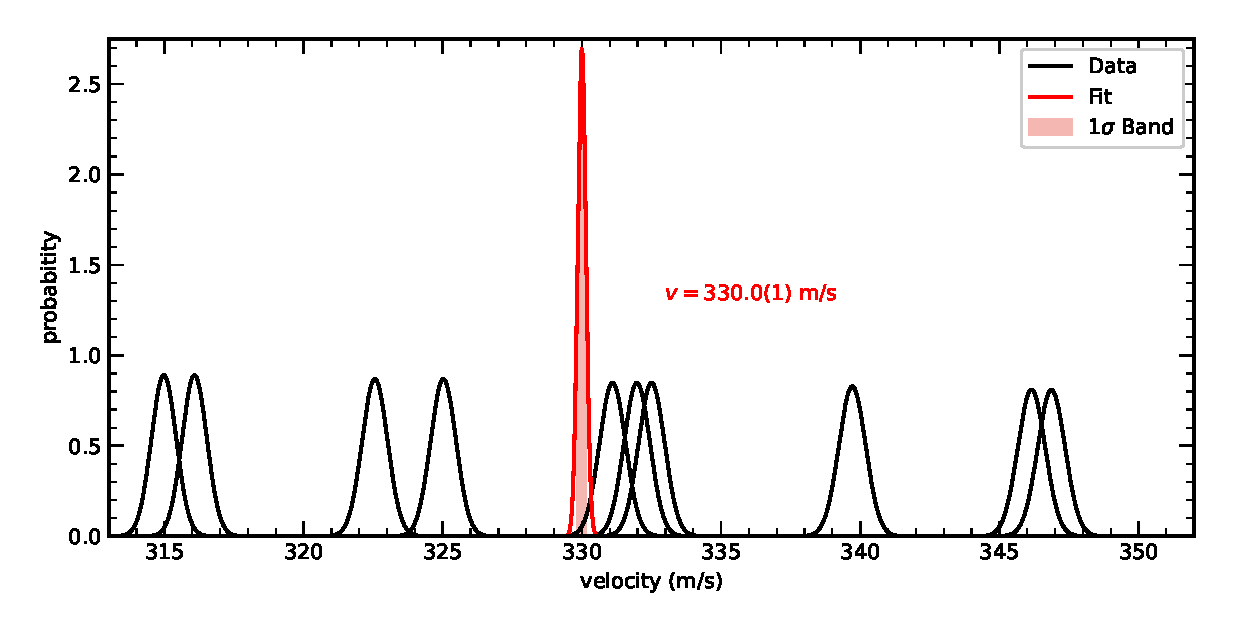
\includegraphics[width=\textwidth]{Versuch4_4.eps}
		\caption{Die gemessenen Geschwindigkeiten wurden als normalisierte Gaußkurven in schwarz auf die Geschwindigkeiten aufgetragen. In Rot der gewichtete Mittelwert, der sich als Überlagerung (und anschließende Normalisierung) der schwarzen Kurven ergibt. Das \( 1\sigma \) Intervall des Mittelwerts wurde farblich hinterlegt.}
		\label{fig:gauss}
	\end{figure}

	Man erhält also \( v = 330.0(1) \unit{\v} \) als besten Schätzwert für die Schallgeschwindigkeit. Der Fehler ist im Vergleich zur berechneten Geschwindigkeit der Laufzeitmethode, da die Unsicherheit in der Zeit aufgrund der Fouriertransformation wegfällt. Es wurden aber Annahmen getroffen, wie zum Beispiel dass das Rohr perfekt Rund sei, welche in der Praxis nicht ganz erfüllt sind und daher zu nicht berücksichtigten Fehlern führen. Um diese zu eliminieren, müsste man den Versuch in einer kontrollierteren Umgebung und mit genauerem Equipment durchführen, um Fehler durch Imperfektionen zu eliminieren.
\end{mybox}
\newpage
\begin{mybox}{Berechnung der Schallgeschwindigkeit}
	Die Schallgeschwindigkeit lässt sich für ideale Gase mithilfe des adiabatischen Kompressionsmoduls berechnen 
	\begin{equation}\label{eqn:cad}
		c_{\text{ad}} = \sqrt{\gamma RT/M}
	\end{equation}
	wobei \( \gamma \approx 1.4 \) der Adiabatenindex, \( R = 8.3143 \unit{J K^{-1} mol^{-1}} \) die allgemeine Gaskonstante, \( T \) die Temperatur und \( M \approx 0.028973 \unit{kg/mol} \) die molare Masse des Gases beschreiben.
	Die Temperatur wurde mittel eines Thermometers auf \( 297(1) \unit{K} \) gemessen. 
	Setzt man nun Werte in \autoref{eqn:cad} ein, erhält man 
	\begin{equation}\label{eqn:cad2}
		c_{\text{ad}} = 345.45(6) \unit{\v}
	\end{equation}
	
	Dieser Geschwindigkeit liegt etwas über den empirisch ermittelten Werten. Im Falle der Laufzeitmessung weicht der gemessene Wert nicht signifikant von \autoref{eqn:cad} ab, was systematische Fehler aber nicht ausschließt. Die Resonanzmethode liefert einen sehr genauen Wert, der zwar mir der Laufzeitmessung gut übereinstimmt, mit \autoref{eqn:cad} nicht vereinbar ist. Entweder der statistische Fehler wurde hier zu klein abgeschätzt, oder es liegen systematische Fehler vor, die das Resultat verfälschen (und wahrscheinlich sogar beides). 
	
	Die Schallgeschwindigkeit lässt sich über mehrere Methoden empirisch ermitteln. Der wesentliche Unterschied zwischen dem Laufzeitverfahren und dem Resonanzverfahren ist, dass Ersteres die Geschwindigkeit direkt misst, während Zweiteres sie indirekt über Interferenz bestimmt. Für die direkte Messung braucht man nur eine Definition der Messgröße (\( v = \Delta s/ \Delta t \)), während die indirekte Messung ein Modell braucht, das die beiden Größen in Verbindung setzt.
	
	Der Adiabatenindex \( \gamma \), auch Wärmekapazitätsverhältnis genannt, wird durch das Verhältnis zwischen der Wärmekapazität eines Gases bei konstantem Druck zur Wärmekapazität bei konstantem Volumen beschrieben. Man kann ihn auch über die Freiheitsgrade des Gases definieren. Er hängt daher von der Temperatur des Gases ab, da diese die freie Bewegung des Gases einschränkt.
	Für Luft gilt \( \gamma \approx 1.4 \) unter der Voraussetzung, das die Temperatur um \( 300 \unit{K} \) liegt.
	
	Aus \( 	\rho c \zeta_0 \omega = p_0 \) und \( \omega = 2\pi f \) folgt für \( \zeta_0 \) und \( v_0 \)
	\begin{align}\label{eqn:zeta}
		\zeta_0 &= \frac{p_0}{2\pi f\rho c} = 3.8854 \cdot 10^{-5} \unit{m} \\
		v_0 &= \zeta_0\omega = \frac{p_0}{2\rho c} = 0.2441 \unit{\v}
	\end{align}
	Substituiert man in der Zustandsgleichung für ideale Gase \( V = m/\rho \) erhält man für die Dichte
	\begin{equation}\label{eqn:density}
		\rho_0 = \frac{p_0M}{RT} = 0.01742 \unit{kg/m^3}
	\end{equation}
\end{mybox}

\end{document}